\documentclass[tikz,border=14pt]{standalone}
\usepackage{helvet}
\renewcommand{\familydefault}{\sfdefault}
\usepackage[T1]{fontenc}
\usetikzlibrary{positioning,fit,calc,backgrounds,arrows.meta,shadows}

% ---------- palette ----------
\definecolor{cBrowser}{HTML}{2563EB}
\definecolor{cServer}{HTML}{0D9488}
\definecolor{cAI}{HTML}{EA580C}
\definecolor{cOut}{HTML}{DB2777}
\definecolor{cInk}{HTML}{1E2433}
\definecolor{cMute}{HTML}{6B7280}

% ---------- styles ----------
\tikzset{
  step/.style={draw=#1, fill=white, line width=1.1pt, rounded corners=9pt,
    minimum width=7.4cm, minimum height=2.2cm, text width=6.8cm, align=left,
    inner sep=9pt, text=cInk, drop shadow={opacity=0.12}},
  badge/.style={circle, fill=#1, text=white, font=\bfseries\small,
    minimum size=0.8cm, inner sep=0pt},
  arrow/.style={-{Stealth[length=3.2mm,width=2.6mm]}, line width=1.5pt, color=cMute!75},
  elabel/.style={fill=white, inner sep=2.5pt, font=\scriptsize\bfseries, text=cMute, rounded corners=2pt},
}
\newcommand{\ttl}[1]{{\bfseries\normalsize #1}\\[2pt]}
\newcommand{\tech}[1]{{\scriptsize\ttfamily\color{cMute}#1}\\[2pt]}

\begin{document}
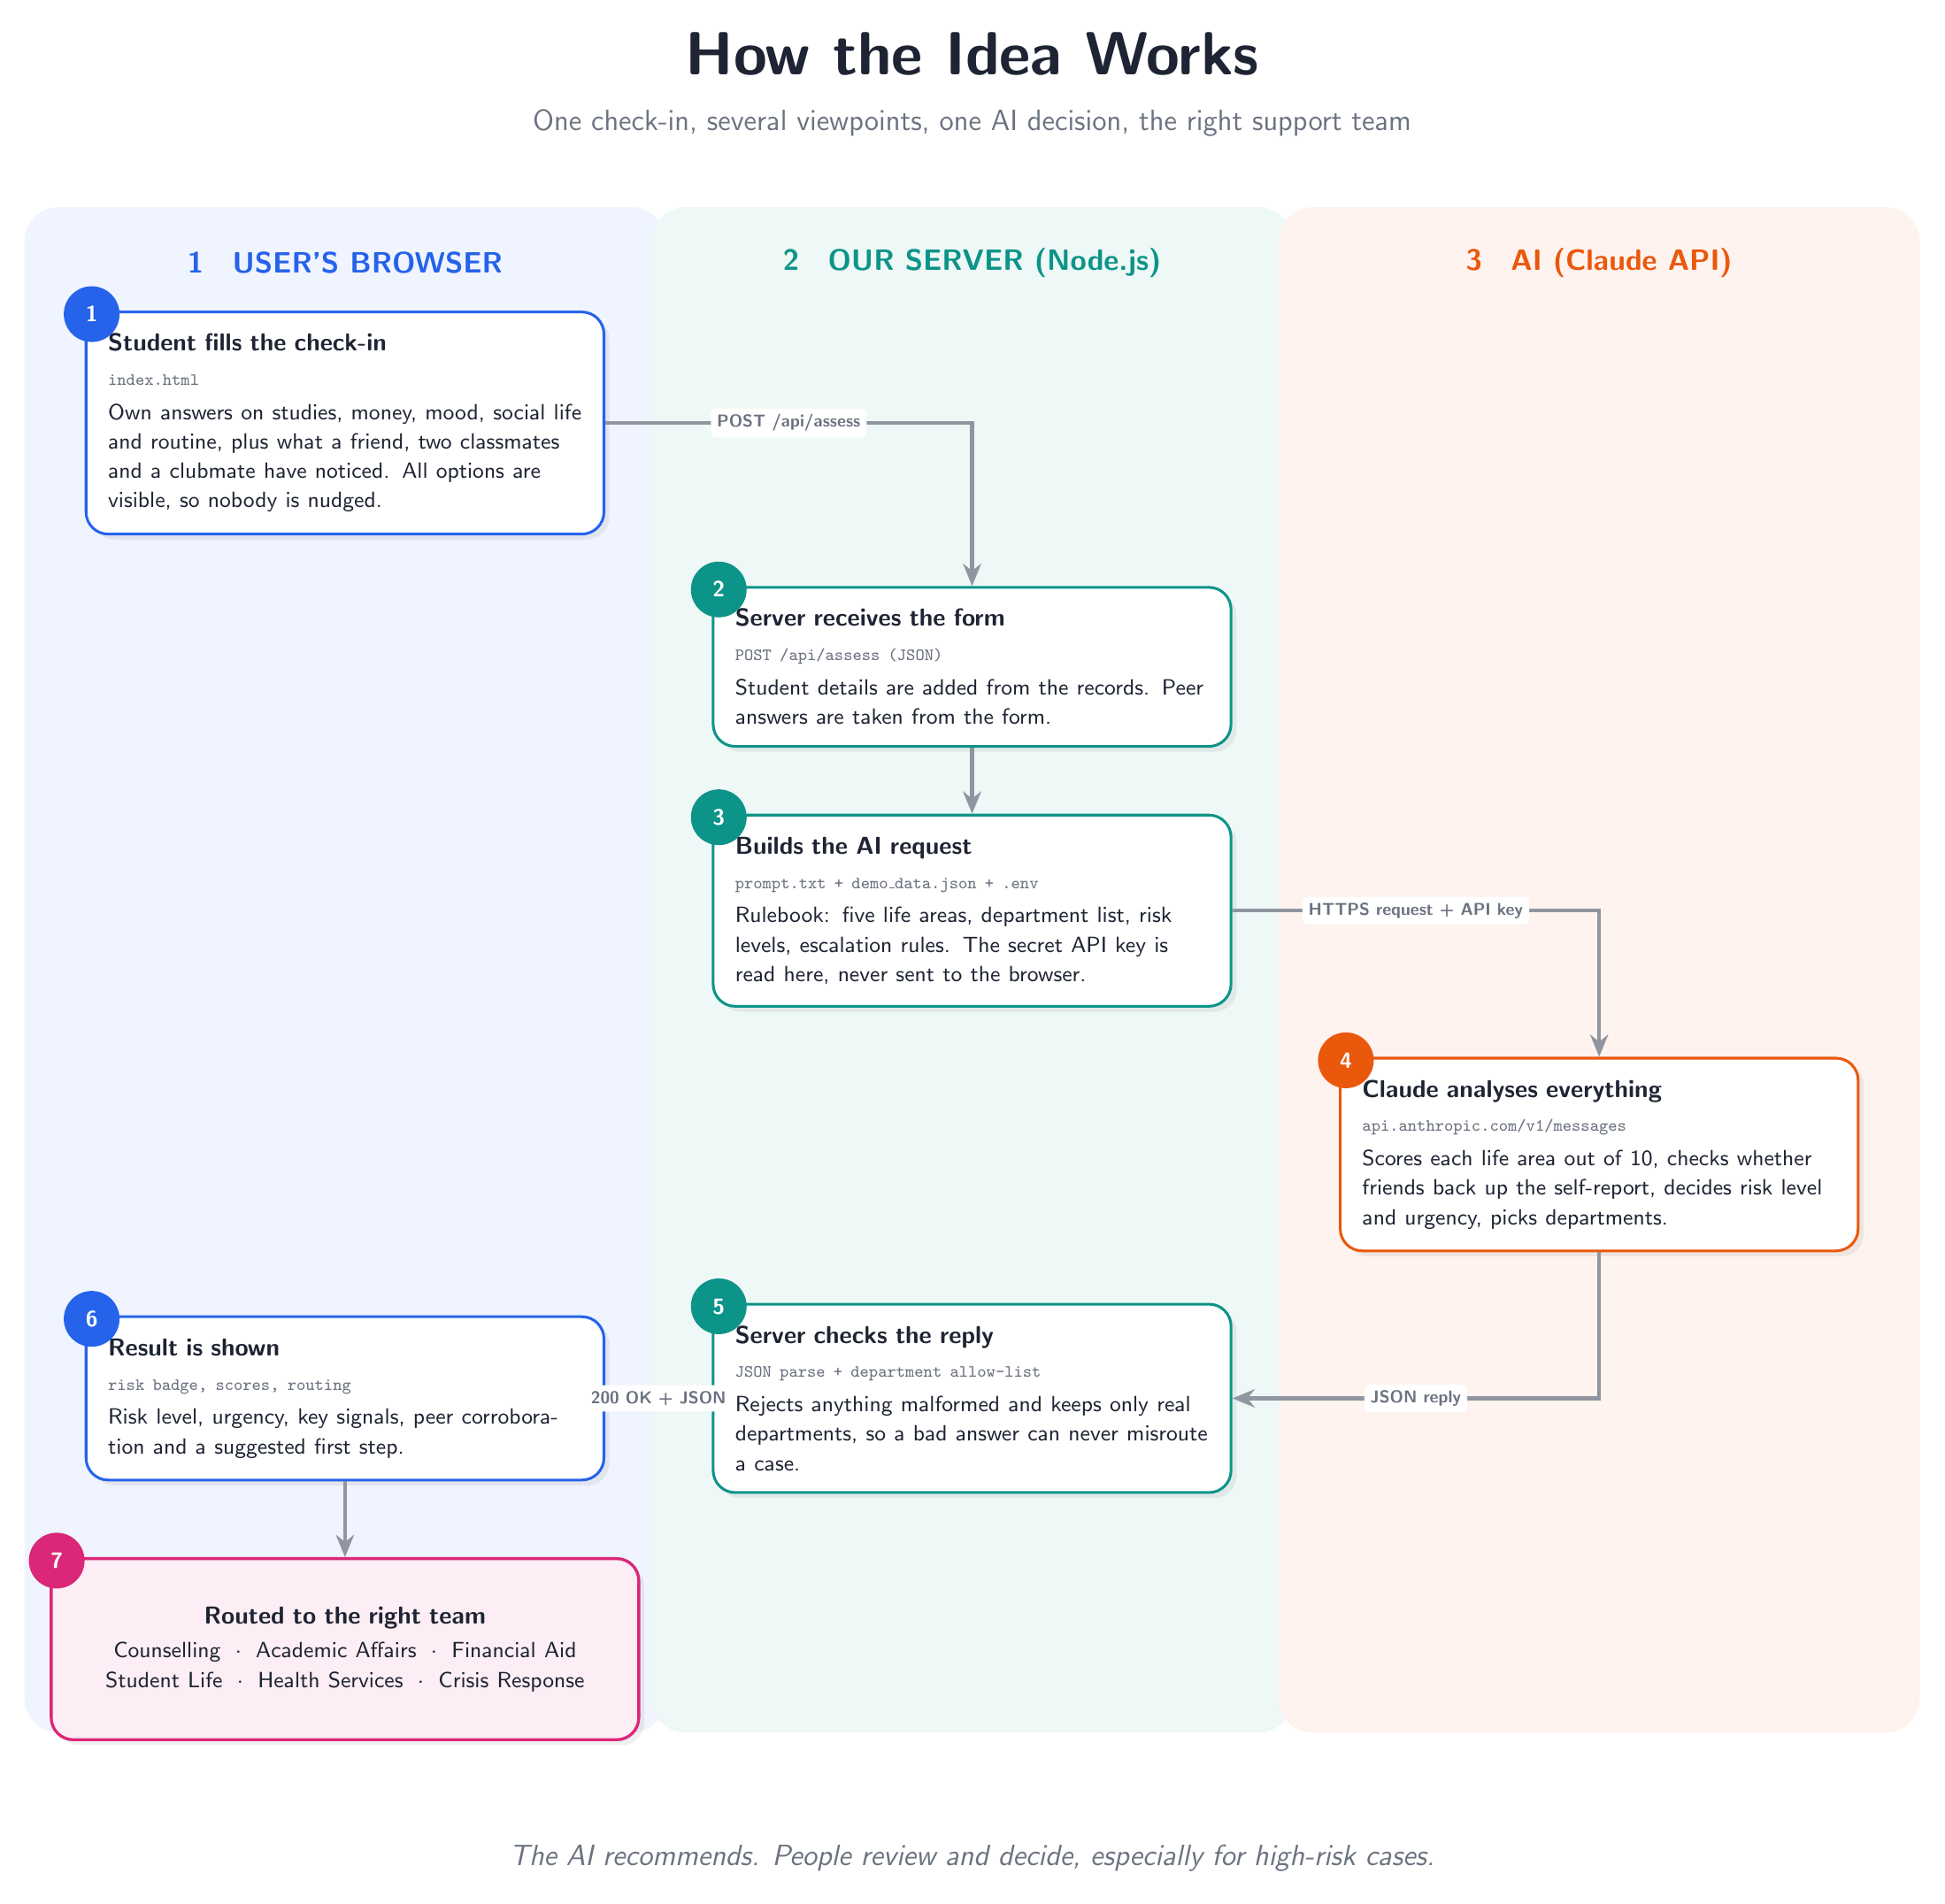
\begin{tikzpicture}[>=Stealth]

  % ---------- title ----------
  \node[font=\Huge\bfseries, text=cInk] at (9,4.9) {How the Idea Works};
  \node[font=\large, text=cMute] at (9,3.9)
    {One check-in, several viewpoints, one AI decision, the right support team};

  % ---------- swim lanes ----------
  \begin{scope}[on background layer]
    \fill[cBrowser!7, rounded corners=14pt] (-4.6,2.7) rectangle (4.6,-19.2);
    \fill[cServer!7,  rounded corners=14pt] (4.4,2.7)  rectangle (13.6,-19.2);
    \fill[cAI!7,      rounded corners=14pt] (13.4,2.7) rectangle (22.6,-19.2);
  \end{scope}
  \node[font=\bfseries\large, text=cBrowser] at (0,1.9) {1\;\; USER'S BROWSER};
  \node[font=\bfseries\large, text=cServer]  at (9,1.9) {2\;\; OUR SERVER (Node.js)};
  \node[font=\bfseries\large, text=cAI]      at (18,1.9) {3\;\; AI (Claude API)};

  % ---------- steps ----------
  \node[step=cBrowser] (b1) at (0,-0.4)
    {\ttl{Student fills the check-in}\tech{index.html}%
     \small Own answers on studies, money, mood, social life and routine, plus what a friend, two classmates and a clubmate have noticed. All options are visible, so nobody is nudged.};

  \node[step=cServer] (s1) at (9,-3.9)
    {\ttl{Server receives the form}\tech{POST /api/assess  (JSON)}%
     \small Student details are added from the records. Peer answers are taken from the form.};

  \node[step=cServer] (s2) at (9,-7.4)
    {\ttl{Builds the AI request}\tech{prompt.txt + demo\_data.json + .env}%
     \small Rulebook: five life areas, department list, risk levels, escalation rules. The secret API key is read here, never sent to the browser.};

  \node[step=cAI] (c1) at (18,-10.9)
    {\ttl{Claude analyses everything}\tech{api.anthropic.com/v1/messages}%
     \small Scores each life area out of 10, checks whether friends back up the self-report, decides risk level and urgency, picks departments.};

  \node[step=cServer] (s3) at (9,-14.4)
    {\ttl{Server checks the reply}\tech{JSON parse + department allow-list}%
     \small Rejects anything malformed and keeps only real departments, so a bad answer can never misroute a case.};

  \node[step=cBrowser] (b2) at (0,-14.4)
    {\ttl{Result is shown}\tech{risk badge, scores, routing}%
     \small Risk level, urgency, key signals, peer corroboration and a suggested first step.};

  % ---------- departments ----------
  \node[draw=cOut, fill=cOut!8, line width=1.2pt, rounded corners=9pt, text width=7.8cm, align=center,
        inner sep=9pt, minimum height=2.6cm, text=cInk, drop shadow={opacity=0.12}] (dep) at (0,-18.0)
    {\textbf{Routed to the right team}\\[3pt]\small
     Counselling \;$\cdot$\; Academic Affairs \;$\cdot$\; Financial Aid\\
     Student Life \;$\cdot$\; Health Services \;$\cdot$\; Crisis Response};

  % ---------- arrows ----------
  \draw[arrow] (b1.east) -| node[elabel, pos=0.25] {POST /api/assess} (s1.north);
  \draw[arrow] (s1.south) -- (s2.north);
  \draw[arrow] (s2.east) -| node[elabel, pos=0.25] {HTTPS request + API key} (c1.north);
  \draw[arrow] (c1.south) |- node[elabel, pos=0.75] {JSON reply} (s3.east);
  \draw[arrow] (s3.west) -- node[elabel] {200 OK + JSON} (b2.east);
  \draw[arrow] (b2.south) -- (dep.north);

  % ---------- step badges ----------
  \foreach \num/\col/\target in {1/cBrowser/b1, 2/cServer/s1, 3/cServer/s2,
                                 4/cAI/c1, 5/cServer/s3, 6/cBrowser/b2} {
    \node[badge=\col] at ($(\target.north west)+(0.1,-0.05)$) {\num};
  }
  \node[badge=cOut] at ($(dep.north west)+(0.1,-0.05)$) {7};

  % ---------- footer ----------
  \node[font=\large\itshape, text=cMute, align=center] at (9,-21)
    {The AI recommends. People review and decide, especially for high-risk cases.};

\end{tikzpicture}
\end{document}
